\subsection{Radius and objective-unit controls}
\label{sec:robustness}
The final control varies the radius while keeping each real-data objective
fixed. The logistic radii are $1,2,4$ and the Poisson radii are
$0.75,1.5,3$. Each radius has a newly computed constrained reference
interval; the Poisson curvature bounds are recomputed on its new domain.
Five matched seeds and objective scales $a\in\{10^{-3},1,10^3\}$ give
360 runs of four methods: FW/AFW with either $M=1$ or $M=U_0/D^2$.
The target for $af$ is $a10^{-5}$, so all conditions use the same
accuracy in original units. No reference or curvature constants are
solver inputs, and certificate initialization reuses the first paid
function, gradient, and LMO evaluations. The 30 unscaled default-radius
baselines agree exactly with their earlier records.

\begin{proposition}[Objective units in halving backtracking]
\label{prop:units}
In exact arithmetic, replace $f$ by $\widetilde f=af+b$, $a>0$, and
$\varepsilon$ by $a\varepsilon$. For FW or AFW, scale $M$ by $a$ and
use identical scale-invariant tie breaking. Then all iterates, accepted
steps, trial counts, and stopping indices are unchanged. In particular,
$M=U_0/D^2$ makes this scaling automatic. Keeping $M$ fixed instead
corresponds to initialization $M/a$ on the original objective.
\end{proposition}
\begin{proof}
Every tangent lower bound transforms as $\widetilde\ell=a\ell+b$,
and $\widetilde G=aG$, $\widetilde U=aU$. Positive scaling preserves
LMO and away-atom comparisons. Inductively $\widetilde L=aL$, so the
ratio of directional gap to $L\norm d^2$, the feasible cap, and the
quadratic acceptance comparison are unchanged. Halving and doubling
commute with positive scaling. The stopping test scales identically.
\end{proof}
This elementary property is an initialization control, not a new
convergence result. The curvature parameters transform as
$\widetilde H_0=aH_0$, $\widetilde H_1=H_1$; strong convexity scales
as $\widetilde\mu=a\mu$.

Both AFW initializations certify all 90 radius/seed/scale conditions
within 1000 updates. FW certifies 30/90 with fixed $M$ and 33/90 with
certificate initialization. These counts include repeated scalings of
the same problems and are not independent replications. At scale one,
the certificate-initialized AFW function-call median increases from
73 to 388 as the logistic radius goes from 1 to 4; all five seeds
still finish. At Poisson radius 3, that median is 1292 and only 1/5
seeds finish within 1000 function calls. Thus success within the update
cap is distinct from success at a fixed function budget.

Objective units can affect more than the final call count. For logistic
radius 1, FW with fixed $M=1$ certifies 0/5 at $a=10^{-3}$ but 5/5 at
$a=1$ and $10^3$. For both certificate-initialized methods, all 60
matched scale comparisons preserve final function/gradient/LMO counts
and stopping outcomes. The maximum relative change in $U/a$ across
the recorded oracle-budget prefixes is below $3.2\cdot10^{-11}$,
using denominator $\max\{10^{-5},U_{a=1}\}$. This compares recorded
certificates and counters, not bitwise equality of complete iterates;
finite precision can change branch decisions in general.

All logistic references are on the constraint boundary. The Poisson
reference has $\ell_1$ norm approximately 0.692 and is interior at
all three radii. Thus this control does not test an active Poisson
constraint. No new dataset or predictive-performance claim is added.
Changing the radius changes both the domain and its original starting
vertex. Certificate initialization is not uniformly faster than the
fixed initialization. Additional AFW active-set work remains separately
counted, and no wall-clock ranking follows.

\begin{table}[htbp]
\centering\small
\caption{Radius controls at objective scale $a=1$, five matched seeds. Each entry gives final successes (out of five); median function calls. Capped failures are included. The cap is 1000 updates, not 1000 function calls. Subscript $1$: $M=1$; subscript $U$: $M=U_0/D^2$.}
\label{tab:robustness}
\begin{tabular}{lrrrr}
\hline
Radius & FW$_1$ & FW$_U$ & AFW$_1$ & AFW$_U$ \\
\hline
\multicolumn{5}{l}{\textbf{breast\_cancer}} \\
$R=1$ & 5; 205 & 5; 161 & 5; 83 & 5; 73 \\
$R=2$ & 0; 1997 & 0; 1999 & 5; 105 & 5; 101 \\
$R=4$ & 0; 1998 & 0; 2000 & 5; 342 & 5; 388 \\
\hline
\multicolumn{5}{l}{\textbf{bike\_poisson}} \\
$R=0.75$ & 0; 2002 & 0; 2003 & 5; 829 & 5; 906 \\
$R=1.5$ & 4; 1804 & 4; 423 & 5; 791 & 5; 635 \\
$R=3$ & 3; 1920 & 2; 1999 & 5; 1085 & 5; 1292 \\
\hline
\end{tabular}
\end{table}

\begin{figure}[htbp]
\centering
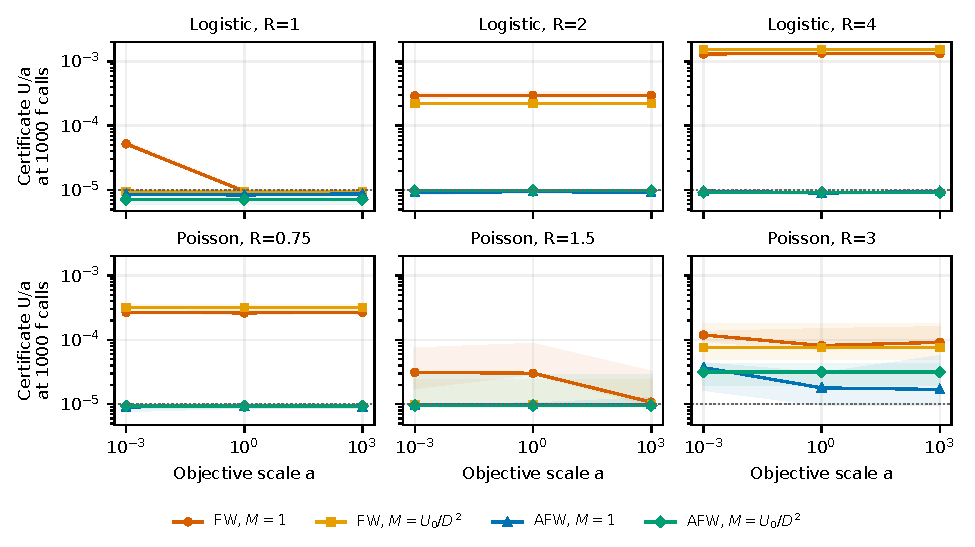
\includegraphics[width=\textwidth]{figures/radius_and_units.pdf}
\caption{Radius and objective-unit controls. Median and interquartile
band of the certificate in original units, $U/a$, after at most 1000
function calls, five matched seeds. The tolerance is $10^{-5}$ in these
units. Completed runs are carried forward; nonterminal runs reach the
displayed budget before the update cap. Lines only connect the three
tested scales. Scaled versions of a problem are paired controls.}
\label{fig:robustness}
\end{figure}
